\chapter{Resultater}

I denne del af rapporten fremlægges projektets resultater fra modultesten, integrationstesten og  accepttesten. Der fokuses på kun få udvalgt resultater, der er vigtige for produktets funktionsdygtighed,  fra hver af de nævnte testtyper. De fulde resultater, der er opnåede under disse tests henvises der til de pågældende bilage. I det følgende præsenteres første hardware resultaterne, der er opnåede i modultesten og integrationstesten efterfulgt af software resultaterne, der opnåede inden for det samme testtype. Tilslut fremvises accepttestens resultater.     

\section{Hardware resultater}
\subsection{Modul resultater}
Under modultesten af hardwaredelen er der opnåede resultater for hver af de testede moduler, se disse resultater i \nameref{bilag6}. En af de kritiske opnåede resultater for hele systemet var resultatet fra strømgeneratoren. Figur \ref{fig:Stromgeneratorload} viser strømproduktion af strømgeneratoren. Her ses at strømmen er konstant, når belastningen varieres op til $10k \Omega$, hvilken er den højeste impedans som et menneskevæv kan levere. Til variering af belastningen er der brugt en variabel modstand.        

\begin{figure}[H] 
\centering
{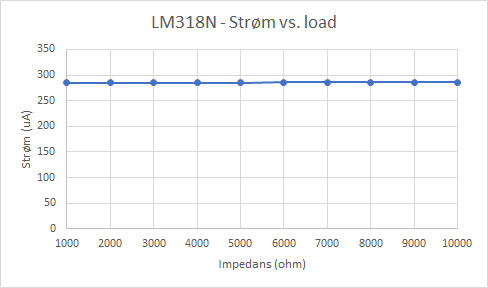
\includegraphics[width=12cm]
{Figure/Stromgeneratorload}}
\caption{Output-strømmen af strømgeneratoren, når belastningen varieres fra $1 - 10k\Omega$}
\label{fig:Stromgeneratorload}
\end{figure}


\pagebreak 

Et andet vigtigt resultatet for hele systemet var resultatet af systemets AA filter. For at afgøre, hvor meget filteret dæmpning skal være, sammensættes alle systemets komponenter for at lave en spektrumanalyse. På \ref{fig:aaspectrum1} kan man aflæse amplituden på den målte signal, samt hvor meget amplituden er dæmpet ved 250kHz, som er den halve samplingfrekvens. Det kan aflæses at signalet er aftaget med 75dB. Dette betyder at systemets AA-filter skal dæmpe signalet yderligere med 15dB  for at opfylde ADC'ens bit range, som 90dB.   

       
\begin{figure}[H] 
\centering
{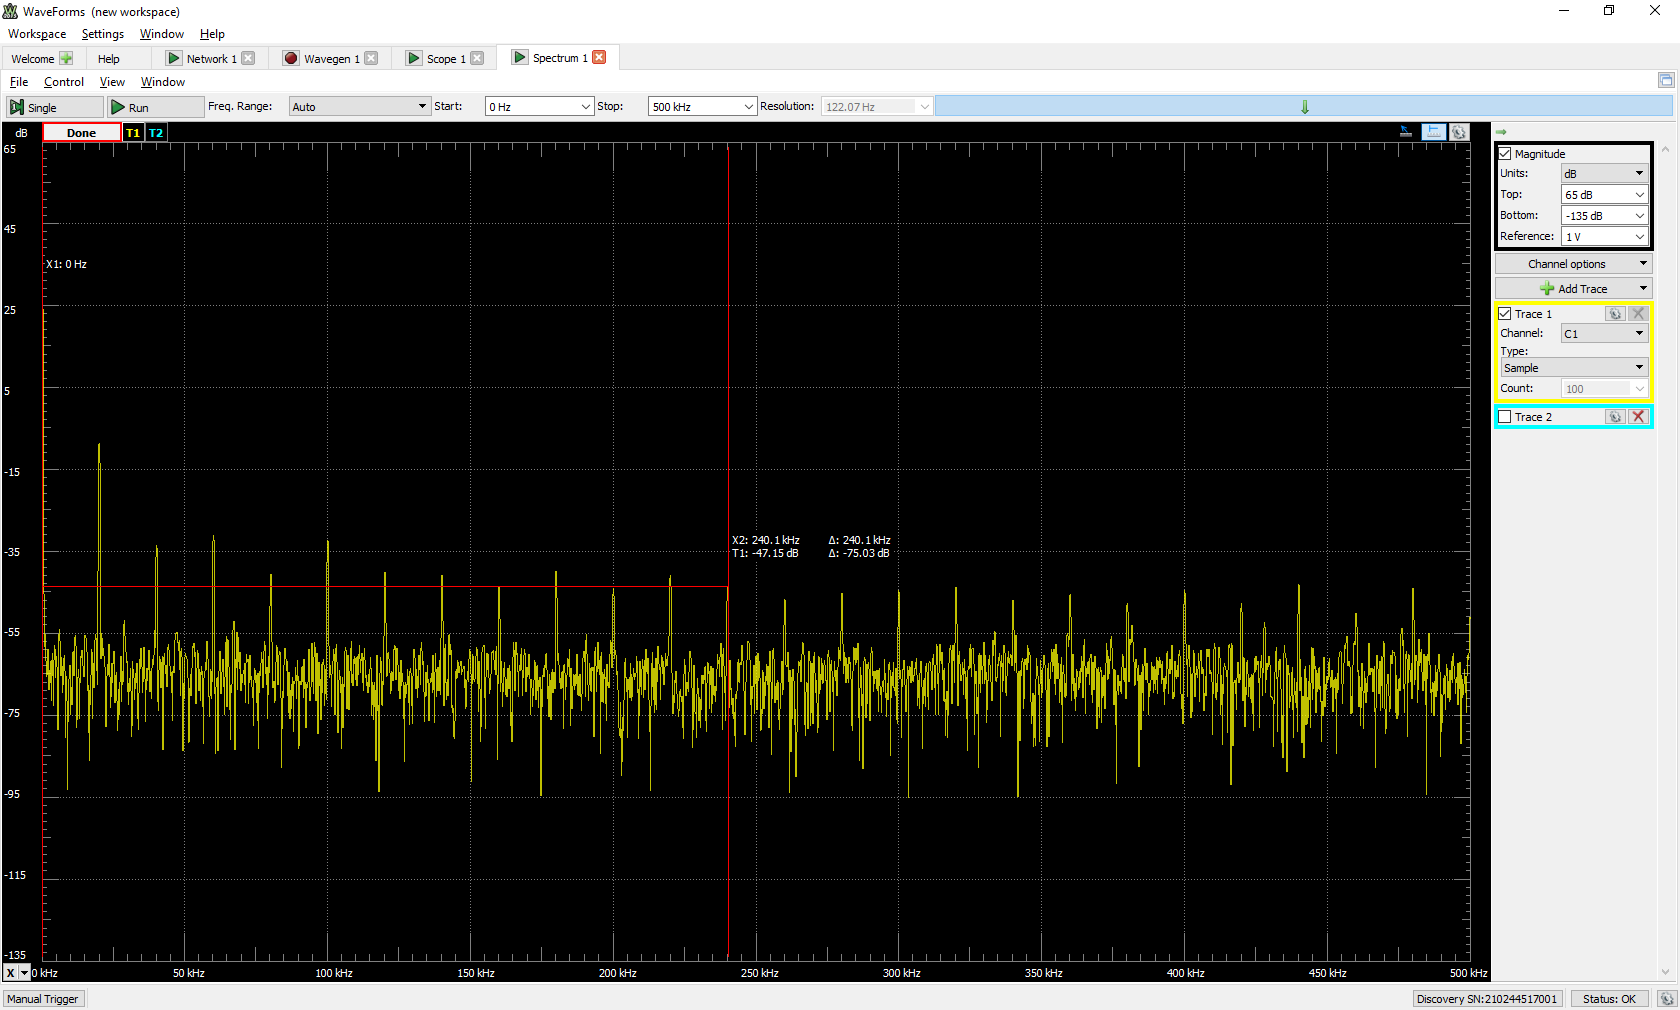
\includegraphics[width=\linewidth]
{Figure/aaspectrum1}}
\caption{Det implementeret frekvensspektrum, som viser at der er en samlet dæmpning på ca. 75dB som skal yderligere dæmpes til 90dB med et 2.ordens lavpasfilter.}
\label{fig:aaspectrum1}
\end{figure}

\pagebreak

Da man nu kender, hvor meget signalet skal dæmpes, designes der en 2. ordens lavpasfilter. På figur \ref{fig:aafiltermodultest} ses at filteret er i stand til at dæmpe et signal med mere end 15dB. 


\begin{figure}[H] 
\centering
{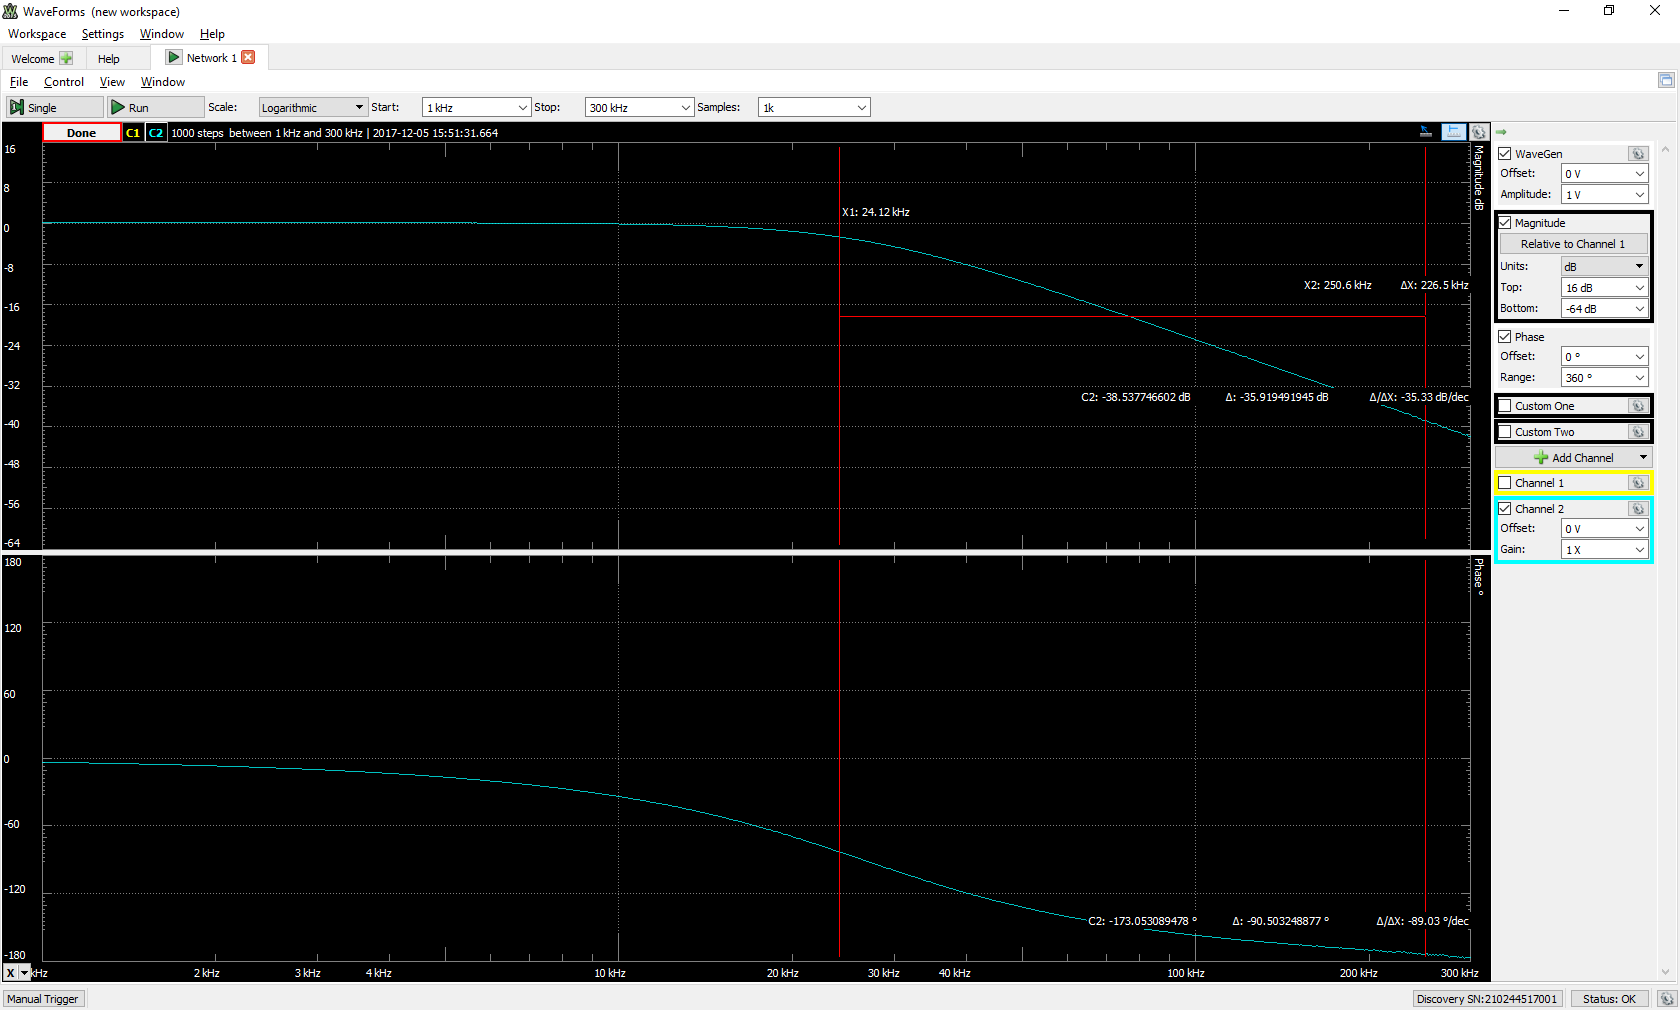
\includegraphics[width=\linewidth]
{Figure/aafiltermodultest}}
\caption{Resultat om filterets virkning fra Network Analyzer i waveforms.}
\label{fig:aafiltermodultest}
\end{figure}



\subsection{Integrationstest}



\section{Software}
\subsection{Modultest}
\subsection{Integrationstest}


\section{Accepttest}

De funktionelle krav som dette projekt har prioriteret højst er de krav, der er defineret i \textit{Must og Should}. Til opfyldelsen af disse krav, er der benyttet use cases, der sammen definerer, hvordan disse krav opnås. De detaljeret testudførsel og resultater kan læses i \nameref{bilag6}. I tabel \ref{AT_UC1} præsenteres use casens resultat udfald. 
  
\begin{longtabu} to \linewidth{@{} c X[l] X[l] X[j] c@{}}
    ~ &	\textbf{Use case nr.} &    \textbf{Krav type} &		\textbf{Testresultat} \\[-1ex]
    \midrule
    ~ & 1 & Funktionelle krav & Godkendt &
    \\ \midrule
   &   2 &   Funktionelle krav & Godkendt   &	
   
\\ \midrule
   &   3 &   Funktionelle krav & Godkendt   &   
   
 \\ \bottomrule
 
\caption{Resultaterne for de funktionelle krav, der er defineret i kravspecifikationen}\\
\label{AT_UC1}
\end{longtabu}


De tre use cases tilsammen opfylder kravene i \textit{Must og Should} i kravspecifikationen med undtagelse krav nummer 9. Se kapitel 7, hvorfor dette krav ikke er opfyldt. 

\pagebreak
\section{Ikke-funktionelle krav}

Tilforskel fra de funktionelle krav er de ikke-funktionelle krav ikke organiseret i use cases. De ikke-funktionelle krav består af punkter, der definerer produktets kvalitetsaspekter. Disse skal være testbart. Herunder opsummeres resultaterne af accepttesen for de ikke-funktionelle krav. 

\begin{longtabu} to \linewidth{@{} c X[l] X[l] X[j] c@{}}
    ~ &	\textbf{Krav nr.} &    \textbf{Krav type} &		\textbf{Testresultat} \\[-1ex]
    \midrule
    ~ & 1 & ikke-funktionelle krav & ej testbart &
    \\ \midrule
   &   2 &   ikke-funktionelle krav & ej testbart   &	
   
\\ \midrule
   &   3 &   ikke-funktionelle krav & ej testbart   &   
   
   \\ \midrule
   &   4 &   ikke-funktionelle krav & Godkendt   &  
   
   
    \\ \midrule
   &   5 &   ikke-funktionelle krav & Godkendt   & 
   
    \\ \midrule
   &   6 &   ikke-funktionelle krav &  ej testbart  & 
   
   
    \\ \midrule
   &   7 &   ikke-funktionelle krav &  ej testbart  & 
     \\ \midrule
   &   8 &   ikke-funktionelle krav & Godkendt  & 
     \\ \midrule
   &   9 &   ikke-funktionelle krav &  ej testbart  &  
   \\ \midrule
    &   10 &   ikke-funktionelle krav &  Godkendt  &  
    
    \\ \midrule
    &   11 &   ikke-funktionelle krav &  Godkendt  &  
   
   
 \\ \bottomrule
 
\caption{Resultaterne for de ikke-funktionelle krav, der er defineret i kravspecifikationen}\\
\label{AT_UC2}
\end{longtabu}

Som det ses i tabel \ref{AT_UC2} er der en del krav, der er mærkeret som ej testbart under accepttesten. Gruppen har været fuld bevidst om at disse krav ikke er testbart, men har alligevel medtaget som et ønsket kvalitets parametre. Dette valg er truffet for at gøre brugeren/kunden opmærksom på, at produktet ikke er testet under de nævnte forhold og dermed skal brugeren være opmærksom på at anvende produktet under disse forhold, der ikke testet.  